\documentclass[12pt,compress,aspectratio=169]{beamer}

\mode<presentation>
{
  \usetheme{metropolis}
  \setbeamersize{text margin left=.8cm,text margin right=.8cm}
%  \setbeamertemplate{navigation symbols}{} % suppress nav bar
%  \setbeamercovered{transparent}
}
\usefonttheme{professionalfonts}
\usepackage{amsmath,bm}
\usepackage{siunitx}
%\usepackage{graphicx}
\usepackage{tikz}
\usepackage{mathpazo}
%\usepackage[scaled]{helvet}
\usepackage{xcolor,colortbl}
%\usepackage{hyperref}

\setmonofont{Liberation Mono}
\setlength{\parskip}{0pt}
\setlength{\itemsep}{0pt}
\renewcommand{\baselinestretch}{1}

\sisetup{
  number-math-rm=\mathnormal,
  per-mode=symbol
}

\title{Topic 6: General Circular Motion}
\subtitle{Advanced Placement Physics}
\author[TML]{Dr.\ Timothy Leung}
\institute{Olympiads School}
\date{December 7, 2019}

\newcommand{\pic}[2]{\includegraphics[width=#1\textwidth]{#2}}
\newcommand{\mb}[1]{\ensuremath\mathbf{#1}}
\newcommand{\eq}[2]{\vspace{#1}{\Large\begin{displaymath}#2\end{displaymath}}}


\begin{document}

\begin{frame}
  \maketitle
\end{frame}


\begin{frame}{Files to Download}
  Please download the following files from the school website if you have not
  already done so:
  \begin{itemize}
  \item\texttt{PhysAP-06-rotMotion-print.pdf}---The ``print version'' of the
    class slides for this topic.
  \item\texttt{PhysAP-06-Homework.pdf}---Homework problems for this topic.
  \end{itemize}
  \vspace{.1in}Please download/print the PDF file for the class slides before
  each class. There is no point copying notes that are already on the slides.
  Instead, focus on things that aren't necessarily on the slides. If you wish
  to print the slides, we recommend printing 4 slides per page.
\end{frame}



\section{Polar Coordinates}

\begin{frame}{Polar Coordinate System in 2D}
  \begin{columns}
    \column{.28\textwidth}
    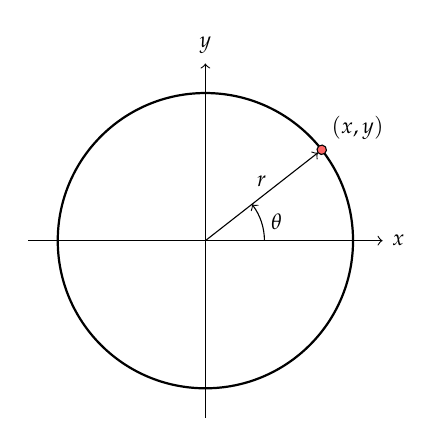
\begin{tikzpicture}[scale=.75]
      \draw[->](-3,0)--(3,0) node[pos=1,right]{\footnotesize$x$};
      \draw[->](0,-3)--(0,3) node[pos=1,above]{\footnotesize$y$};
      \draw[thick] (0,0) circle(2.5);
      \begin{scope}[rotate=38]
        \draw[->] (0,0)--(2.42,0) node[midway,above]{\footnotesize$r$};
        \draw[fill=red!60] (2.5,0) circle(.08)
        node[above right]{\footnotesize$(x,y)$};
      \end{scope}
      \draw(1,0)[->] arc(0:38:1) node[midway,right]{\footnotesize$\theta$};
    \end{tikzpicture}
    \column{.7\textwidth}
    \begin{itemize}
    \item Cartesian coordinate system $\mb{x}(x,y)$ is not the only way to
      describe the position of an object
    \item For circular motion, \textbf{polar coordinates} are better
    \item Position described by $\mb{r}(r,\theta)$
      \begin{itemize}
      \item $r$ is distance from the origin
      \item $\theta$ is the standard angle, measured counter-clockwise from the
        positive $x$ axis
      \end{itemize}
    \item Cartesian and polar coordinates are related by:

      \vspace{-.3in}{\large
        \begin{align*}
          x&=r\cos\theta\\
          y&=r\sin\theta
        \end{align*}
      }
    \end{itemize}
  \end{columns}
\end{frame}


\begin{frame}{Cylindrical Coordinates in 3D}
  \begin{columns}
    \column{.45\textwidth}
    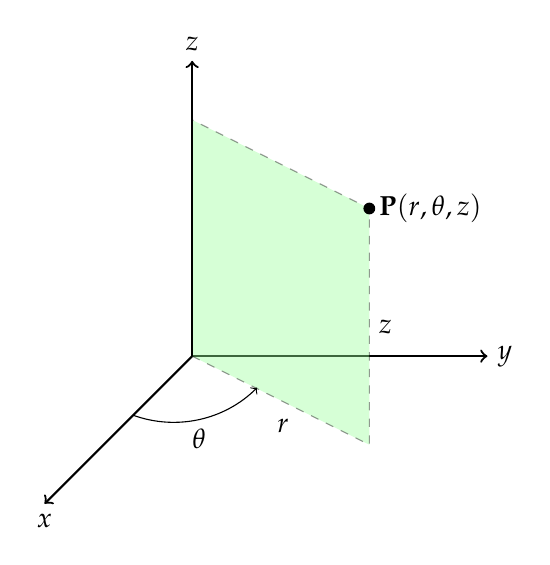
\begin{tikzpicture}[scale=.75]
      \draw[thick,->](0,0)--(-2.5,-2.5)node[pos=1,below]{$x$};
      \draw[thick,->](0,0)--(5,0)   node[pos=1,right]{$y$};
      \draw[dashed,fill=green!40,opacity=.4](0,0)--(3,-1.5)
      node[pos=.6,below left,opacity=1]{$r$}--(3,2.5)
      node[midway,right,black,opacity=1]{$z$}--(0,4);
      \fill[black](3,2.5) circle(.1) node[right]{$\mb{P}(r,\theta,z)$};
      \draw[->] (-1,-1) arc(-110:-45:2) node[midway,below]{$\theta$};
      \draw[thick,->](0,0)--(0,5) node[pos=1,above]{$z$};
    \end{tikzpicture}

    \column{.55\textwidth}
    One way to extend the coordinates coordinate system into 3D. This is called
    the \textbf{cylindrical coordinate system}. Note that the discussions for
    this topic focuses on $xy$ plane. Since the $z$-axis is linearly
    independent of the $xy$ plane, motion along that direction is independent.
  \end{columns}
\end{frame}


\begin{frame}{Rigid Body Motion}{Angular Position and Angular Velocity}
  \vspace{.2in}
  \begin{columns}
    \column{.32\textwidth}
    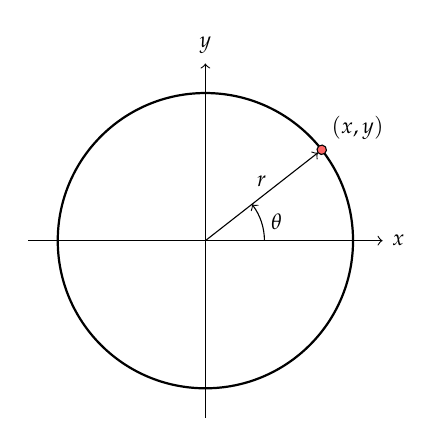
\begin{tikzpicture}[scale=.75]
      \draw[->](-3,0)--(3,0) node[pos=1,right]{\footnotesize$x$};
      \draw[->](0,-3)--(0,3) node[pos=1,above]{\footnotesize$y$};
      \draw[thick] (0,0) circle(2.5);
      \begin{scope}[rotate=38]
        \draw[->] (0,0)--(2.42,0) node[midway,above]{\footnotesize$r$};
        \draw[fill=red!60] (2.5,0) circle(.08)
        node[above right]{\footnotesize$(x,y)$};
      \end{scope}
      \draw(1,0)[->] arc(0:38:1) node[midway,right]{\footnotesize$\theta$};
    \end{tikzpicture}
    
    \column{.68\textwidth}
    For constant $r$, \textbf{angular position} $\theta$ determines an object's
    position as a function of time:
      
    \eq{-.2in}{
      \boxed{\theta=\theta(t)}
    }
    
    \textbf{Angular velocity} $\omega$ (or \textbf{angular frequency}) is its
    time derivative
      
    \eq{-.2in}{
      \boxed{\omega(t)=\frac{d\theta(t)}{dt}=\dot{\theta}}
    }

    $\theta$ is measured in \si{radians}, and $\omega$ in \si{rad/\s}
  \end{columns}
\end{frame}



\begin{frame}{Rigid Body Motion}{Angular Velocity}
  \begin{columns}
    \column{.35\textwidth}
    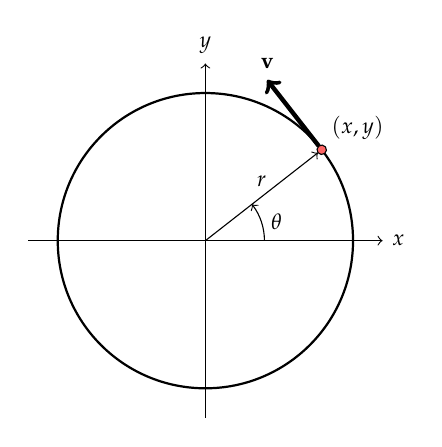
\begin{tikzpicture}[scale=.75]
      \draw[->](-3,0)--(3,0) node[pos=1,right]{\footnotesize$x$};
      \draw[->](0,-3)--(0,3) node[pos=1,above]{\footnotesize$y$};
      \draw[thick] (0,0) circle(2.5);
      \begin{scope}[rotate=38]
        \draw[->] (0,0)--(2.42,0) node[midway,above]{\footnotesize$r$};
        \draw[fill=red!60] (2.5,0) circle(.08)
        node[above right]{\footnotesize$(x,y)$};
        \draw[ultra thick,->](2.5,.08)--(2.5,1.5)
        node[pos=1,above]{\footnotesize$\mb{v}$};
      \end{scope}
      \draw(1,0)[->] arc(0:38:1) node[midway,right]{\footnotesize$\theta$};
    \end{tikzpicture}

    \column{.65\textwidth}

    Velocity $\mb{v}$ and angular velocity $\bm{\omega}$ are related by the
    cross product with the position vector $\mb{r}$:

    \eq{-.25in}{
      \boxed{\mb{v}=\bm{\omega}\times\mb{r}}
    }

    \vspace{-.15in}If you are uncomfortable with the vector notation, the
    scalar form may be more useful to you:
    
    \eq{-.3in}{
      \boxed{v=r\omega}
    }    
    \begin{itemize}
    \item\vspace{-.25in}$\mb{v}$ is tangent to circle, and
      perpendicular to $\mb{r}$
    \item $\bm{\omega}$ is \emph{out of the page} if $\mb{v}$ is
      counterclockwise, and
    \item $\bm{\omega}$ is \emph{into the page} if $\mb{v}$ is clockwise
    \item Visualizing $\bm{\omega}$ will take some practice, but it is
      mathematically rigorious
    \end{itemize}
  \end{columns}
\end{frame}



\begin{frame}{Rigid Body Motion}{Angular Velocity}
  \begin{columns}
    \column{.35\textwidth}
    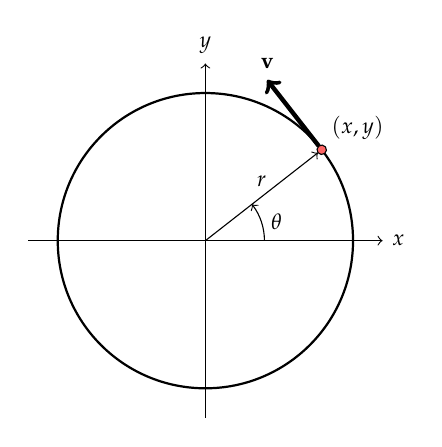
\begin{tikzpicture}[scale=.75]
      \draw[->](-3,0)--(3,0) node[pos=1,right]{\footnotesize$x$};
      \draw[->](0,-3)--(0,3) node[pos=1,above]{\footnotesize$y$};
      \draw[thick] (0,0) circle(2.5);
      \begin{scope}[rotate=38]
        \draw[->] (0,0)--(2.42,0) node[midway,above]{\footnotesize$r$};
        \draw[fill=red!60] (2.5,0) circle(.08)
        node[above right]{\footnotesize$(x,y)$};
        \draw[ultra thick,->](2.5,.08)--(2.5,1.5)
        node[pos=1,above]{\footnotesize$\mb{v}$};
      \end{scope}
      \draw(1,0)[->] arc(0:38:1) node[midway,right]{\footnotesize$\theta$};
    \end{tikzpicture}

    \column{.65\textwidth}
    For constant angular velocity $\omega$, the motion is \textbf{periodic}. Its
    \textbf{frequency} and \textbf{period} are given by:

    \eq{-.3in}{
      \boxed{f=\frac{\omega}{2\pi}}\quad
      \boxed{T=\frac{2\pi}{\omega}}\quad
        \boxed{f=\frac{1}{T}}
    }
    
    $T$ is in seconds (\si{\s}) and $f$ is in hertz (\si{\hertz})
  \end{columns}
\end{frame}



\begin{frame}{Rotating Object Without Slipping}
  A tire with radius $r$ rolls along the road with an angular velocity $\omega$
  \emph{without slipping}. (This is a very common case for analysis.)  What
  is its velocity $v$
  \begin{enumerate}[a.]
  \item at the contact between the ground and the tire?
  \item at the center?
  \item at the top of the tire?
  \end{enumerate}

  \vspace{-.4in}
  \begin{center}
    \hspace{1in}
    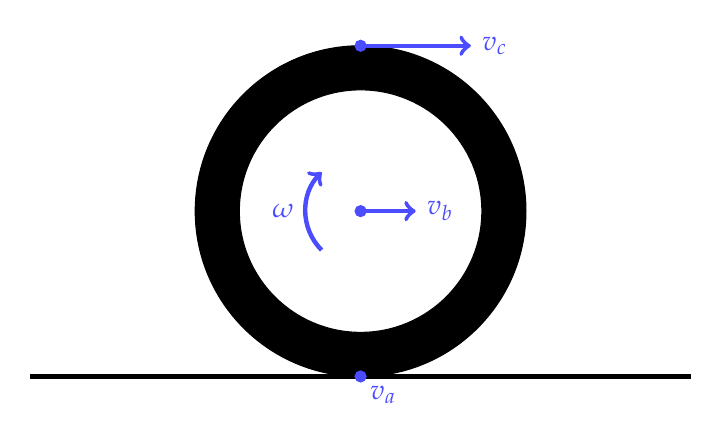
\begin{tikzpicture}[scale=.7]
      \draw[fill=black](0,0) circle(3);
      \draw[fill=white](0,0) circle(2.2);
      \draw[ultra thick](-6,-3)--(6,-3);
      \draw[ultra thick,blue!70,->](-.707,-.707) arc(225:135:1)
      node[midway,left]{$\omega$};
      \draw[fill=blue!70,blue!70](0,-3) circle(.1) node[below right]{$v_a$};
      \draw[fill=blue!70,blue!70](0,0) circle(.1);
      \draw[ultra thick,blue!70,->](0,0)--(1,0) node[pos=1,right]{$v_b$};
      \draw[fill=blue!70,blue!70](0,3) circle(.1);
      \draw[ultra thick,blue!70,->](0,3)--(2,3) node[pos=1,right]{$v_c$};
    \end{tikzpicture}
  \end{center}
\end{frame}

\begin{frame}{Rigid Body Motion}{Angular Acceleration}
  The derivative of $\omega$ with respect to time gives us
  \textbf{angular acceleration}, which has a unit of \si{rad/\second^2}:

  \eq{-.2in}{
    \boxed{\alpha=\dot{\omega}=\ddot{\theta}}
  }

  Similar to the relationship between velocity and angular velocity,
  \textbf{tangential acceleration} $a_\theta$ is related to angular acceleration
  $\alpha$ by the radius $r$:
    
  \eq{-.2in}{
    \boxed{a_\theta(t)=\dot{v}=r\dot{\omega}=r\alpha}
  }
    
  For \emph{uniform} circular motion, $\omega$ is constant, and therefore
  $\alpha_\theta=0$
\end{frame}


\begin{frame}
  \frametitle{Kinematics in the Angular Direction}
  \framesubtitle{These Should Look Familiar}
  For constant $\alpha$, the kinematic equations are just like in linear
  motion:
  
  \begin{columns}
    \column{.55\textwidth}
    {\Large
      \begin{align*}
        \theta&=\theta_0 + \omega_0 t + \frac{1}{2}\alpha t^2\\
        \theta&=\theta_0+ \frac{\omega_0+\omega}{2} t
      \end{align*}
    }
    
    \column{.45\textwidth}
    {\Large
      \begin{align*}
        \omega&= \omega_0+ \alpha t\\
        \omega^2& = \omega_0^2+ 2\alpha(\theta-\theta_0)
      \end{align*}
    }
  \end{columns}
  Of course, if $\alpha$ is \emph{not} constant, we will have to integrate
\end{frame}



\begin{frame}{A Simple Example}
  \textbf{Example 1:} An object moves in a circle with angular acceleration
  \SI{3.}{rad/\s^2}. The radius is \SI{2.}{\metre} and it starts from rest. How
  long does it take for this object to finish a circle?
\end{frame}



\begin{frame}{Nothing is Ever \emph{That} Simple}
  Remember, even when $\alpha=0$, we still have a centripetal acceleration
  $a_r$ for any circular motion

  \eq{-.2in}{
    \boxed{a_r=\frac{v^2}{r}=\omega^2r=\frac{4\pi^2r}{T^2}=4\pi^2rf^2}
  }

  And with the centripetal acceleration, there is also a
  \textbf{centripetal force}

  \eq{-.2in}{
    \boxed{F_r=ma_r=\frac{mv^2}{r}}
  }
\end{frame}



\begin{frame}{Acceleration: The General Case}
  \begin{columns}
    \column{.2\textwidth}
    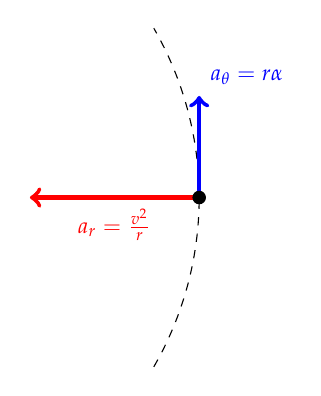
\begin{tikzpicture}[scale=4.3]
      %\draw[dashed] (0,0) circle(3);
      \draw[dashed] (.866,-.5) arc(-30:30:1);
      \draw[ultra thick, red,->] (1,0)--(.5,0)
      node[pos=0.5,below]{\footnotesize $a_r=\frac{v^2}{r}$};
      \draw[ultra thick, blue,->] (1,0)--(1,.3)
      node[pos=1,above right]{\footnotesize $a_\theta=r\alpha$};
      \fill (1,0) circle(.02);
    \end{tikzpicture}
    
    \column{.8\textwidth}
    \begin{itemize}
    \item In general circular motion, there are two components of acceleration:
      \begin{itemize}
      \item\textcolor{red}{\textbf{Centripetal acceleration} $a_r$} depends on
        radius of curvature $r$ and instantaneous speed $v$
      \item \textcolor{blue}{\textbf{Tangential acceleration} $a_\theta$}
        depends on radius $r$  and angular acceleration $\alpha$
      \end{itemize}
    \item Most of the cases in AP Physics are uniform circular motion
    \end{itemize}
  \end{columns}
\end{frame}


\begin{frame}{How to Solve Circular Motion Problems}
  A two-step process:
  \begin{enumerate}
  \item Is there any circular motion?
  \item If so, the condition for circular motion is:

    \eq{-.2in}{
      \mb{F}_\mathrm{provided}=\mb{F}_\mathrm{required}
    }
    \begin{itemize}
    \item The \emph{provided} force comes from FBD
    \item The \emph{required} force comes from the centripetal equation we have
    \end{itemize}
  \end{enumerate}
\end{frame}



\begin{frame}{Example: Horizontal Motion}
  \begin{columns}
    \column{.4\textwidth}
    \pic{1}{puck-on-table.png}
    
    \column{.6\textwidth}
    \textbf{Example 2:} In the figure on the left, a mass
    $m_1=\SI{3.}{\kilo\gram}$ is rolling around a frictionless table with
    radius $R=\SI{1.}{\metre}$. with a speed of \SI{2.}{\metre\per\second}.
    What is the mass of the weight $m_2$?
  \end{columns}
\end{frame}


\begin{frame}{Another Example: Exit Ramp}
  \textbf{Example 3:} A car exits a highway on a ramp that is banked at
  $15^\circ$ to the horizontal. The exit ramp has a radius of curvature of
  \SI{65}{\metre}. If the conditions are extremely icy and the driver cannot
  depend on any friction to help make the turn, at what speed should the driver
  travel so that the car will not skid off the ramp? What if there is friction?
\end{frame}



\begin{frame}{Vertical Circles}
  \begin{itemize}
  \item Uniform circular motion with a horizontal path is straightforward
  \item For vertical motion:
    \begin{itemize}
    \item Generally not solvable by dynamics
    \item We can use conservation of energy to solve for $\mb{v}$
    \item Then use the equation for centripetal force to find other forces
    \end{itemize}
  \item\textbf{Remember:} If it is impossible to get the required centripetal
    force, then it could not continue the circular motion
  \end{itemize}
\end{frame}



\begin{frame}{Example Problem}
  \textbf{Example 4:} A cord is tied to a pail of water, and the pail is swung
  in a vertical circle of \SI{1.}{\metre}. What must be the minimum velocity of
  the pail be at its highest point so that no water spills out?

  \begin{enumerate}[(a)]
  \item\SI{3.1}{\metre\per\second}
  \item\SI{5.6}{\metre\per\second}
  \item\SI{20.7}{\metre\per\second}
  \item\SI{100.5}{\metre\per\second}
  \end{enumerate}
\end{frame}


\begin{frame}{Example: Roller Coaster}
  \textbf{Example 5:} A roller coaster car is on a track that forms a circular
  loop, of radius $R$, in the vertical plane. If the car is to maintain contact
  with the track at the top of the loop (generally considered to be a good
  thing), what is the minimum speed that the car must have at the bottom of the
  loop. Ignore air resistance and rolling friction.
  \begin{enumerate}[(a)]
  \item $\sqrt{2gR}$
  \item $\sqrt{3gR}$
  \item $\sqrt{4gR}$
  \item $\sqrt{5gR}$
  \end{enumerate}
\end{frame}


\begin{frame}{Example}
  \textbf{Example 6:} A stone of mass $m$ is attached to a light strong string
  and whirled in a \emph{vertical} circle of radius $r$. At the exact bottom of
  the path, the tension of the string is three times the weight of the stone.
  The stone's speed at that point is given by:
  \begin{enumerate}[(a)]
  \item $2\sqrt{gR}$
  \item $\sqrt{2gR}$
  \item $\sqrt{3gR}$
  \item $4gR$
  \end{enumerate}
\end{frame}


\section{Torque}

\begin{frame}{Torque and Rotational Equilibrium}
  Let's consider this question:
  \begin{center}
    \fbox{
      \begin{minipage}{.7\textwidth}
        Two people stand on a board of uniform density. One person has a mass of
        \SI{50}{\kilo\gram} and stands \SI{10}{\metre} away from the fulcrum
        (pivot). The second person has a mass of \SI{65}{\kilo\gram}. How far
        away from the fulcrum would the second person have to stand for the
        system to have to be in equilibrium?
      \end{minipage}
    }
  \end{center}
\end{frame}



\begin{frame}{Equation of Motion}{Newton's Second Law}
  Recall Newton's second law of motion for objects with constant mass:
    
  \eq{-.2in}{
    \mb{F}_\mathrm{net}=m\mb{a}
  }
  \begin{itemize}
  \item Is it also true for \emph{circular} motion?
  \item If a net force $\mb{F}_\mathrm{net}$ causes a mass to accelerate
    (linearly), what causes a mass to go into circular motion?
  \end{itemize}

  \uncover<2->{
    \vspace{.3in}
    \textbf{Answer:} We need to introduce a few concepts first\ldots
  }
\end{frame}



\begin{frame}{Torque}
  I have a rod on a table, and with my fingers, I push the two ends of the rod
  with equal force $\textcolor{red}{F}$. \textbf{What happens?}
  \begin{center}
    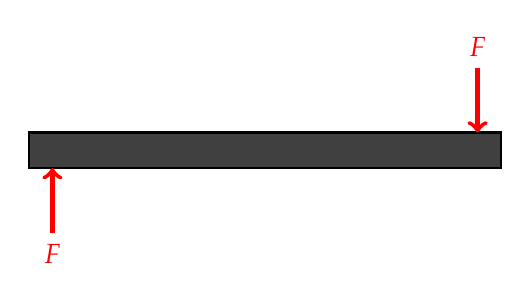
\begin{tikzpicture}[scale=1.5]
      \fill[black!75,draw=black,thick] (-2,-.15) rectangle (2,.15);
      \draw[ultra thick,red,->](-1.8,-.7)--(-1.8,-.15) node[pos=0,below]{$F$};
      \draw[ultra thick,red,->]( 1.8, .7)--( 1.8, .15) node[pos=0,above]{$F$};
    \end{tikzpicture}
  \end{center}
  $\mb{F}_\mathrm{net}=\mb{0}$, therefore $\mb{a}=\mb{0}$. But (obviously) it
  won't stay still either!
\end{frame}



\begin{frame}{What is Torque?}
  \textbf{Torque} (or \textbf{moment}) is the tendency for a force to change
  the rotational motion of a body.
  
  \begin{itemize}
  \item A force $\mb{F}_a$ acting at a point some distance $\mb{r}$ (called the
    \textbf{moment arm}) from a \textbf{fulcrum} (or \textbf{pivot}) at an angle
    $\phi$ between $\mb{F}_a$ and $\mb{r}$
  \item e.g.\ the force to twist a screw
%  \item In the example below, an applied force $\mb{F}_a$ is applied away from
%    the pivot at an angle $\phi$. This generates a torque around the pivot.
  \end{itemize}
  \begin{center}
    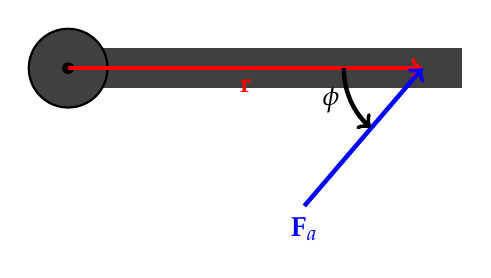
\begin{tikzpicture}[scale=2.5]
      \fill[black!75,draw=black!75] (0,-.1) rectangle (2,.1);
      \fill[black!75,draw=black,thick] (0,0) circle (.2);
      \fill[black] (0,0) circle (.03);
      \draw[ultra thick,red,->](0,0)--(1.8,0) node[midway,below]{$\mb{r}$};
      \draw[ultra thick,blue,->](1.2,-.7)--(1.8,0)node[pos=0,below]{$\mb{F}_a$};
      \draw[ultra thick,->] (1.4,0) arc(180:229:.4)
      node[midway,left]{$\phi$};
    \end{tikzpicture}
  \end{center}
\end{frame}



\begin{frame}{Torque}
  In scalar form, we can express torque $\bm{\tau}$ as the force $\mb{F}_a$,
  the \textbf{moment arm} $\mb{r}$ and the angle $\phi$ between $\mb{F}_a$ and
  $\mb{r}$:

  \eq{-.2in}{
    \boxed{\tau=rF_a\sin\phi}
  }
  
  In vector form, we use the cross-product:

  \eq{-.2in}{
    \boxed{\bm{\tau}=\mb{r}\times\mb{F}_a}
  }
  \begin{center}
    \begin{tabular}{l|c|c}
      \rowcolor{pink}
      \textbf{Quantity} & \textbf{Symbol} & \textbf{SI Unit} \\ \hline
      Torque        & $\bm{\tau}$ & \si{\newton\metre} \\
      Applied force & $\mb{F}_a$  & \si{\newton} \\
      Moment arm (from fulcrum to force) & $\mb{r}$ & \si{\metre}\\
      Angle between force and moment arm & $\phi$ & (no units)
    \end{tabular}
  \end{center}
\end{frame}



\begin{frame}{Torque}
  Going back to the example question:
  \begin{center}
    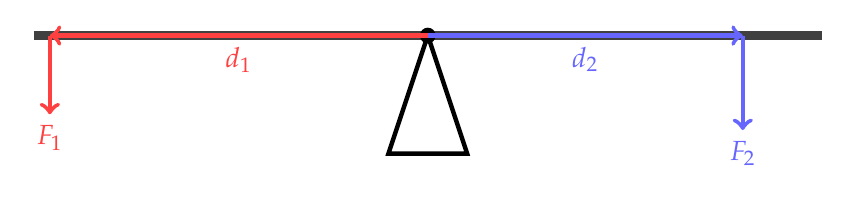
\begin{tikzpicture}
      \fill[black!75,draw=black!75] (-5,-.05) rectangle (5,.05);
      \fill (0,0) circle (.1);
      \draw[ultra thick](0,0)--(.5,-1.5)--(-.5,-1.5)--(0,0);
      \uncover<2->{
        \draw[ultra thick,red!75,->](0,0)--(-4.8,0) node[pos=.5,below]{$d_1$};
        \draw[ultra thick,red!75,->](-4.8,0)--(-4.8,-1)node[pos=1,below]{$F_1$};
      }
      \uncover<3->{
        \draw[ultra thick,blue!60,->](0,0)--(4,0) node[pos=.5,below]{$d_2$};
        \draw[ultra thick,blue!60,->](4,0)--(4,-1.2) node[pos=1,below]{$F_2$};
      }
    \end{tikzpicture}
  \end{center}
  \begin{itemize}
  \item<2->$F_1$ will rotate the board counter clockwise
  \item<3->$F_2$ will rotate the board clockwise
  \item<4->The beam will remain static (in equilibrium) if

    \eq{-.2in}{ F_1d_1=F_2d_2 }
  \end{itemize}
\end{frame}


\begin{frame}{Rotational Equilibrium}
  Just like \textbf{translational equilibrium} is when the force acting on an
  object is zero:
  
  \eq{-.3in}{
    \mb{F}=\mb{0}
  }

  An object is in \textbf{rotational equilibrium} when the
  net torque acting on it is zero:

  \eq{-.3in}{
    \bm{\tau}=\mb{0}
  }

  Note that it doesn't mean that the object isn't rotating, it just means that
  the object's rotational state isn't changing, i.e. $\alpha=0$
\end{frame}



\begin{frame}{Example Problem}
  \textbf{Example 7a:} Find the net torque on point C.

  \vspace{-.2in}
  \begin{center}
    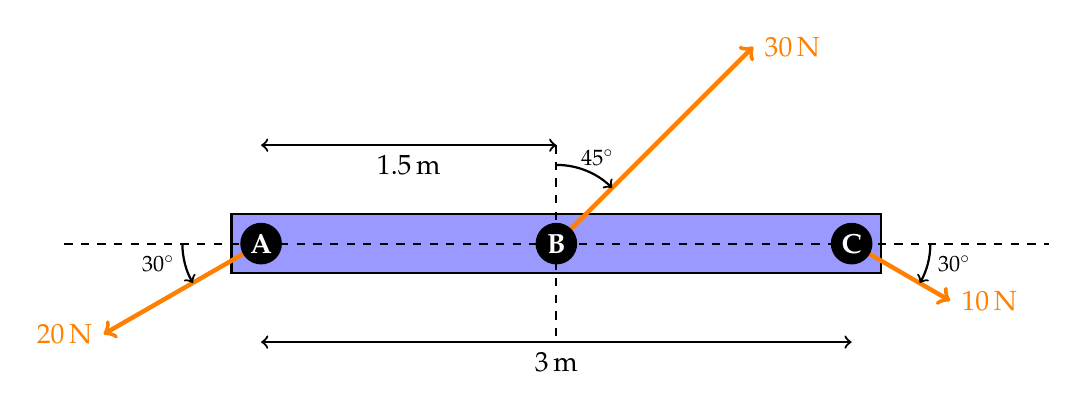
\begin{tikzpicture}[scale=2.5]
      \fill[blue!40!white,draw=black,thick] (-1.65,-.15) rectangle (1.65,.15);
      \draw[thick,<->](-1.5,-.5)--(1.5,-.5) node[midway,below]{\SI{3.}{m}};
      \draw[thick,<->](-1.5,.5)--(0,.5) node[midway,below]{\SI{1.5}{m}};
      \draw[dashed,thick](-2.5,0)--(2.5,0);
      \draw[dashed,thick](0,.5)--(0,-.5);
      \draw[ultra thick,orange,->](0,0)--(1,1)node[pos=1,right]{\SI{30}{N}};
      \draw[thick,->](0,.4)arc(90:45:.4)
      node[pos=.7,above]{\footnotesize\ang{45}};
      \draw[ultra thick,orange,->](-1.5,0)--(-2.3,-.46)
      node[pos=1,left]{\SI{20}{\newton}};
      \draw[thick,->](-1.9,0) arc(180:210:.4)
      node[midway,left]{\footnotesize\ang{30}};
      \draw[ultra thick,orange,->](1.5,0)--(2,-.29)
      node[pos=1,right]{\SI{10}{\newton}};
      \draw[thick,->](1.9,0) arc(0:-30:.4)
      node[midway,right]{\footnotesize\ang{30}};
      \fill[black,draw=black,thick] (-1.5,0) circle(.1);
      \fill[black,draw=black,thick] (   0,0) circle(.1);
      \fill[black,draw=black,thick] ( 1.5,0) circle(.1);
      \node(A) at (-1.5,0) {\color{white}\textbf{A}};
      \node(B) at (0,0) {\color{white}\textbf{B}};
      \node(C) at (1.5,0) {\color{white}\textbf{C}};
    \end{tikzpicture}
  \end{center}
  \uncover<2->{
    \textbf{Example 7b:} Now find the net torque on A.
  }
\end{frame}



\section{Angular Momentum}

\begin{frame}{Angular Momentum}
  \vspace{.15in}
  \begin{columns}
    \column{.77\textwidth}
    Consider a mass $m$ connected to a massless beam rotates with speed $v$ at
    a distance $r$ from the center (shown on the right). It has an
    \textbf{angular momentum} ($L$) of
    
    \eq{-.2in}{
      \boxed{\mb{L}=\mb{r}\times\mb{p}}
    }
    
    \vspace{-.1in}Expanding the terms in the definition:
    
    \eq{-.4in}{
      \mb{L}=\mb{r}\times(m\mb{v})=m\mb{r}\times(\bm{\omega}\times\mb{r})
      =mr^2\bm{\omega}
    }
    
    \vspace{-.2in}Which gives us:
    
    \eq{-.3in}{
      \boxed{\mb{L}=I\bm{\omega}}
    }
    
    \vspace{-.2in}The quantity $I$ is called the \textbf{moment of inertia}.
    
    \column{.23\textwidth}
    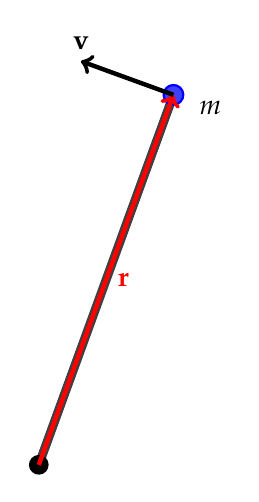
\begin{tikzpicture}[scale=2.5]
      \begin{scope}[rotate=70]
        \fill[black!75,draw=black!75] (0,-.02) rectangle (2,.02);
        \fill[blue!75,draw=blue,thick] (2,0) circle(.05);
        \node(M) at (2,-.2) {$m$};
        \fill[black] (0,0) circle (.05);
        \draw[ultra thick,red,->](0,0)--(2,0)node[pos=.5,right]{$\mb{r}$};
        \draw[ultra thick,->](2,0)--(2,.5)node[pos=1,above]{$\mb{v}$};
      \end{scope}
    \end{tikzpicture}
  \end{columns}
\end{frame}


\begin{frame}{Moment of Inertia}
  A single particle:
  
  \eq{-.2in}{
    \boxed{I=r^2m}
  }

  A collection of particles:

  \eq{-.2in}{
    \boxed{I=\sum r_i^2m_i}
  }

  Continuous distribution of mass:

  \eq{-.2in}{
    \boxed{I=\int r^2dm}
  }
\end{frame}


\begin{frame}{Moment of Inertia}
  \begin{center}
    \pic{.7}{mic.png}
  \end{center}
\end{frame}



\begin{frame}{Angular Momentum and Moment of Inertia}
  \begin{itemize}
  \item Linear and angular momentum have very similar expressions
    
    \eq{-.2in}{
      \mb{p}=m\mb{v}\quad\quad\quad \mb{L}=I\bm{\omega}
    }
  \item Just as $\mb{p}$ describes the overall \emph{translational} state of a
    physical system, $\mb{L}$ describes its overall \emph{rotational} state
  \item In that case, momentum of inertia $I$ can be considered an object's
    ``rotational mass''
  \end{itemize}
\end{frame}



\begin{frame}{Conservation of Angular Momentum}

  \eq{-.1in}{
    \bm{\tau}=\mb{r}\times\mb{F}=\mb{r}\times\frac{d\mb{p}}{dt}
    =\frac{d(\mb{r}\times\mb{p})}{dt}\;\;\longrightarrow\;\;
%      \tau=rF=rm\frac{dv}{dt}=\frac{d(rmv)}{dt}\quad\longrightarrow\quad
%    \end{displaymath}
%    \begin{displaymath}
    \boxed{\bm{\tau} =\frac{d\mb{L}}{dt}}
  }
  \begin{itemize}
  \item If the net torque on a system is zero, then the rate of
    change of angular momentum is zero, and we say that the angular momentum is
    conserved. 
  \item e.g.\ When an ice skater starts to spin and draws his arms inward.
    Since angular momentum is conserved, decreasing $r$ means increasing
    $\omega$
  \item If moment of inertia $I$ is constant in time, the net torque is given
    by:

    \eq{-.2in}{
      \boxed{\bm{\tau}=I\bm{\alpha}}
    }
  \end{itemize}
\end{frame}



\begin{frame}{Example Problem}
  \textbf{Example 8:} A skater extends her arms (both arms!), holding a
  \SI{2.}{\kilo\gram} mass in each hand. She is rotating about a vertical axis
  at a given rate. She brings her arms inward toward her body in such a way that
  the distance of each mass from the axis changes from \SI{1.}{\metre} to
  \SI{.50}{\metre}. Her rate of rotation (neglecting her own mass) will?
\end{frame}



\begin{frame}{Last Example}
  \textbf{Example 9:} A \SI{1.}{\kilo\gram} mass swings in a vertical circle
  after having been released from a horizontal position with zero initial
  velocity. The mass is attached to a massless rigid rod of length
  \SI{1.5}{\metre}. What is the angular momentum of the mass, when it is in its
  lowest position?
\end{frame}


\section{Rotational Kinetic Energy}

\begin{frame}{Rotational Kinetic Energy}
  To find the kinetic energy of a rotating system of particles (discrete number
  of particles, or continuous mass distribution), we sum (or integrate) the
  kinetic energy of the individual particles:
    
  \vspace{-.3in}{\Large
    \begin{align*}
      K&=\sum_i\frac{1}{2}m_iv_i^2=\frac{1}{2}\left(\sum_i m_ir_i^2\right)\omega^2\\
      K&=\int\frac{1}{2}v^2dm=\frac{1}{2}\left(\int r^2dm\right)\omega^2
    \end{align*}
  }
  
  It's no surprise that in both case, rotational kinetic energy is given by:
  
  \eq{-.25in}{
    \boxed{K=\frac{1}{2}I\omega^2}
  }
\end{frame}



\begin{frame}{Kinetic Energy of a Rotating System}
  The total kinetic energy of a rotating system is the sum of its translational
  and rotational kinetic energies at its center of mass:

  \eq{-.2in}{
    \boxed{K=\frac{1}{2}mv_\mathrm{CM}^2+\frac{1}{2}I_\mathrm{CM}\omega^2}
  }
  
  In this case, $I_\mathrm{CM}$ is calculated at the center of
  mass. For simple problems, we only need to compute rotational kinetic energy
  at the pivot:

  \eq{-.2in}{
    \boxed{K=\frac{1}{2}I_\mathrm{P}\omega^2}
  }
  
  In this case, the $I_\mathrm{P}$ is calculated at the pivot.
  \textbf{IMPORTANT:} $I_\mathrm{CM}\neq I_\mathrm{P}$
\end{frame}
\end{document}
